\begin{ProjectEuler}[Multiples of $3$ and $5$]{1}

If we list all the natural numbers below 10 that are multiples of $3$ or $5$, we get $3$, $5$, $6$ and $9$. The sum of these multiples is $23$.
\medskip

\noindent Find the sum of all the multiples of $3$ or $5$ below $1000$.

\end{ProjectEuler}

It is straight forward to iterate over the first $1000$ numbers and check for divisibility.

\begin{pythoncode}
	def divisible_by_3_or_5(limit = 1000):
	    count = 0
	    for num in xrange(1, limit):
	        if num%3 == 0 or num%5 == 0:
	            count += num
	    return count
\end{pythoncode}
%
The code above takes on average \SI{12}{\micro\s} to run. Well under the arbitary \SI{1}{\s} rule. However we can do better, a small improvement
is to allow for different numbers than $3$ or $5$ and also allow for a customizable range. 
%
\begin{pythoncode}
	def numbers_divisible(divisors=[3, 5], start=0, stop=100):
	    count = 0
	    for num in xrange(start, stop):
	        for d in divisors:
	            if num % d == 0:
	                count += num
	                break
	    return count
\end{pythoncode}
%
It could seem the above code is quite fast however running \verb|numbers_divisible([3, 5], 0, 10**9)| takes about \SI{450}{\s} to run. 
This is painfully slow, but also expected since the code runs in $\mathcal{O}(n)$. As we shall see we can make the code run in constant time. 
%
\paragraph*{Improved algorithm for two numbers}
%
The first step is to count the number of numbers divisible by 3, then 5. 
However adding these two will give the incorrect answer, we can see why by listing the first few numbers.
$[3, 6, 9, 15]$ and $[5, 10, 15]$. So every number which is divisble by 3 and 5 is counted twice. \Cref{fig:PE1-venn-2} visualizes this.
%
\begin{figure}[h!tbp]
	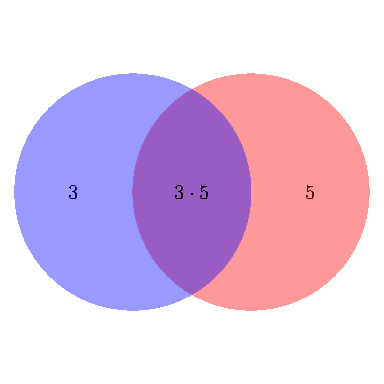
\includegraphics[scale=1, trim={0.25cm 1.25cm 0.25cm 1.25cm}, clip]{Images/Project-Euler-001-Venn-Diagram-2.pdf}
	\caption{}
	\label{fig:PE1-venn-2}
\end{figure}
% 
\begin{pythoncode}
    div_by_3 = [3*i for i in range(int(999/3))]
    div_by_5 = [5*i for i in range(int(999/5))]
    div_by_3_and_5 = [15*i for i in range(int(999/15))]
    return div_by_3 + div_by_5 - div_by_3_and_5
\end{pythoncode}
%
This is slightly faster than the naive implementation. However we can find a closed formula for the number of numbers
divisble by 3, or any other number. The closed formula for the first $n$ numbers are\footnote{See \url{https://en.wikipedia.org/wiki/1_\%2B_2_\%2B_3_\%2B_4_\%2B_\%E2\%8B\%AF} for further details.}
%
\begin{align*}
	0 + 1 + \cdots + (m-1) + m = \frac{m(m+1)}{2}
\end{align*}
%
To find the sum of the natural numbers starting at some number $n$ up to some number $m$ we can subtract the sum of numbers up to $n-1$. 
%
\begin{align*}
	  n + (n+1) + \cdots +(m-1) + m
	= \frac{m(m+1)}{2} - \frac{(n-1)n}{2}
	= \frac{1}{2}(m+n)(m-n+1)
\end{align*} 
Since $3 + 6 + 9 + 12 + \cdots = 3 (1 + 2 + 3 + \cdots)$ we can just multiply the above formula by $3$ to sum the multiples of $3$. 
However we have to make sure we are not multiplying numbers larger than $1000$. So we can not let $m$ be $1000$ and sum up a thousand multiples of $3$.
The largest of these would be $3 \cdot 1000$ which is 3 times as large as the limit. One solution is to take $m = 999/3$. 


If we are summing over multiples of $k$, then the upper limit would be $(text{limit}-1)/k$ rounded down.

One problem with this code can be seen with the $[6, 9]$. The code removes multiples of $6 \cdot 9 = 56$ however the 
first value that is counted twice is $18$. One way to solve this is to divide the product by the lowest common divisor (gcd). 
So we would have $56/\gcd(6,9) = 56/3 = 18$.
%	
\begin{pythoncode}
	from fractions import gcd
	def sum_divisible_by_k(k, start, limit):
    	stop = int((limit-1)/float(k))
    	return k*(stop+start)*(stop-start+1)/2

	def divisible_by_a_or_b(num_a, num_b, start=0, limit=100):
	    divisors = [num_a, num_b]
	    total = 0
	    for divisor in divisors:
	        total += sum_divisible_by_k(divisor, start, limit)
	    product = divisors[0]*divisors[1]/gcd(a, b)
	    return total - sum_divisible_by_k(product, start, limit)
\end{pythoncode}
%
For values up to $10^5$ the improved version runs around $4500$ times faster. However as stated this function runs in constant time
so a speed comparison is not really necessary. We have now done the \emph{silly} speed improvements. 
%
\paragraph*{More than two numbers}

There are some bumps to work out for the generalized version. We shall start looking into the simplest case $[2, 3, 5]$. We can visualize the double counting as follows
%
%
\begin{figure}[h!tbp]
	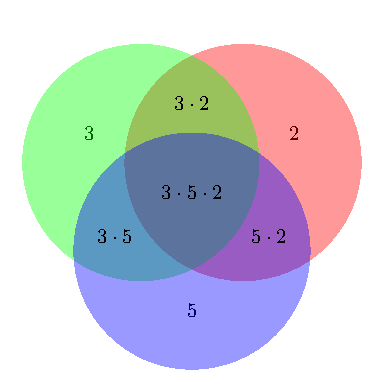
\includegraphics[scale=1, trim={0.25cm 0.25cm 0.25cm 0.75cm}, clip]{Images/Project-Euler-001-Venn-Diagram-3.pdf}
	\caption{}
	\label{fig:PE1-venn-3}
\end{figure}
% 
As we can see from \cref{fig:PE1-venn-3} we have to remove the multiples of $2\cdot 3, 2\cdot 5$ and $3 \cdot 5$. However removing these
will remove too many values. As an exercise you can check that $60$ is missing if we do not add the multiples of $2 \cdot 3 \cdot 5$. 

The next problem to work out is multiples. Take $[2, 3, 8]$, there is no need to add $8$ once we have added $2$. The following code
removes all multiples, all doubles and sorts the divisors. 
%
\begin{pythoncode}
def remove_multiples(divisors):
    new_divisors = []
    divisors = sorted(set(divisors))
    for divisor in divisors:
        if not any(divisor % d == 0 for d in new_divisors):
            new_divisors.append(divisor)
    return new_divisors
\end{pythoncode}
%
The final problem is that we still have to divide by the greatest common divisor. However we now have to perform this on a list of numbers.
Luckily the $\gcd$ functions is additive so that $\gcd(a, b, c) = \gcd( \gcd(a, b), c)$. Since we this be done quite a few times
I will use memoization and save some calculation. 
%
\begin{pythoncode}
gcd_dict = defaultdict(int)
def gcd_list(numbers):
    numbers_len = len(numbers)
    a = perm[0]
    for i in range(1, numbers_len):
        b = perm[i]
        if gcd_dict[(a, b)] == 0:
            gcd_dict[(a, b)] = gcd(a, b)
        a = gcd_dict[(a, b)]
    return a
\end{pythoncode}
%
The final code in all it's glory can now be written as
%
\begin{pythoncode}
def sum_divisible_ny_numbers(numbers, start, stop):
    divisors = remove_multiples(numbers)

    total = 0
    for divisor in divisors:
        total += sum_divisible_by_k(divisor, start, stop)

    k = -1
    for i in range(2, len(divisors)+1):
        for perm in combinations(divisors, i):
            product = reduce(mul, perm)/gcd_list(perm)
            total += k*sum_divisible_by_k(product, start, stop)
        k *= -1
    return int(total)
\end{pythoncode}
%
The running time of this algorithm is $\mathcal{O}(2^{d})$ where $d$ is the number of unique numbers to check for. This is also the reason we take time to remove duplicates
and multiples of values. 

% \bibliographystyle{amsalpha}
% \bibliography{../REFF}

%%% Local Variables: 
%%% mode: latex
%%% TeX-master: "../Project-Euler.tex"
%%% End: 